\documentclass{exam}

\usepackage{units} 
\usepackage[fleqn]{amsmath}
\usepackage{float}
\usepackage{mdwlist}
\usepackage{booktabs}
\usepackage{caption}
\usepackage{fullpage}
\usepackage{enumerate}
\usepackage{graphicx}

% \usepackage{2in1, lscape} 

\everymath{\displaystyle}

\author{}
\date{January 22, 2014}
\title{Statistics \\ Week One}

\begin{document}

\maketitle
\tableofcontents

  \section{Exercise 50}
  If you do a histogram with a bin width of 100, the distribution looks like there
  is a normal distribution.

  \begin{figure}[H]
    \centering
    \includegraphics{figures/ex50_histogram_100.eps}
    \caption{Exercise 50 Histogram (bin width 100)}
  \end{figure}

  Here's the five number summary:
  \begin{table}[H]
    \centering
    \begin{tabular}{rr}
      \toprule
      Min.    & 651 \\
      1st Qu. & 788 \\
      Median  & 861 \\
      3rd Qu. & 905 \\
      Max.    & 1020 \\
      \bottomrule
    \end{tabular}
    \caption{Exercise 50 Summary}
  \end{table}

  The mean is smaller than the median:
  \begin{table}[H]
    \centering
    \begin{tabular}{rr}
      \toprule
      Mean    & 848 \\
      Median  & 861 \\
      \bottomrule
    \end{tabular}
    \caption{Exercise 50 mean and median}
  \end{table}

  The gaps are bigger on the low end:
  \begin{table}[H]
    \centering
    \begin{tabular}{lr}
      \toprule
      median to first quartile & 73 \\
      median to third quartile & 44 \\
      \midrule
      median to minimum & 210 \\
      median to maximum & 159 \\
      \bottomrule
    \end{tabular}
    \caption{Exercise 50 Gaps}
  \end{table}

  You can also see this in the box plot:
  \begin{figure}[H]
    \centering
    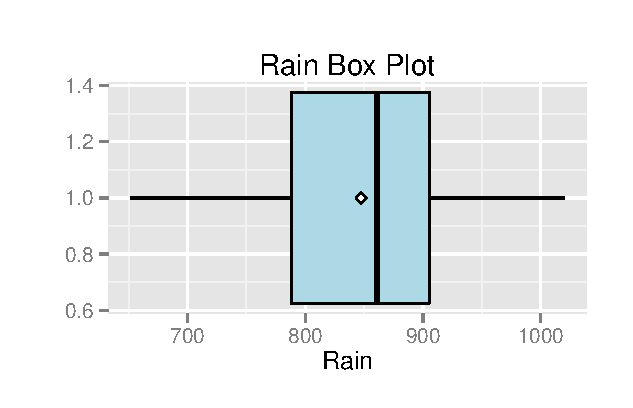
\includegraphics{figures/ex50_box.eps}
    \caption{Exercise 50 box plot}
  \end{figure}

  A histogram with smaller bin width shows that the distribution is left skewed.
  \begin{figure}[H]
    \centering
    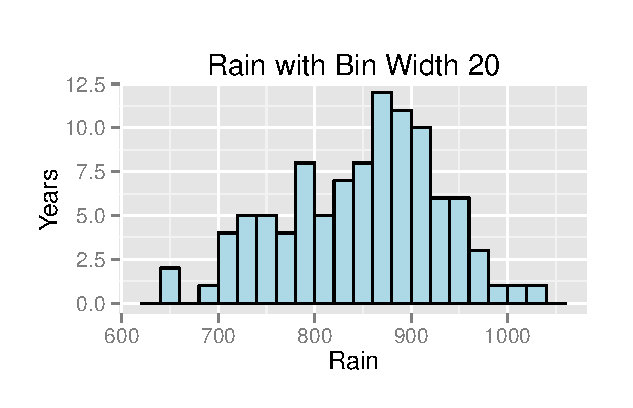
\includegraphics{figures/ex50_histogram_20.eps}
    \caption{Exercise 50 Histogram (bin width 20)}
  \end{figure}

\end{document}

